\documentclass[
journal=jacsat, % for undefined journal
manuscript=article]{achemso}

\newcommand*{\mycommand}[1]{\texttt{\emph{#1}}}

% Bilder
\graphicspath{{images/}}     % Ordner, aus dem die Bilder geladen werden
\usepackage{float}
\usepackage{graphicx} % Bilder
\usepackage{color} % Farben
%\DeclareGraphicsExtensions{.pdf,.png,.jpg, .gif} % bevorzuge pdf-Dateien
\usepackage{subfig}

%\captionsetup[subfigure]{margin=0pt, parskip=0pt, hangindent=0pt, indention=0pt, singlelinecheck=true,  %labelformat=parens}

%\usepackage[all]{hypcap} % Beim Klicken auf Links zum Bild und nicht zu Caption gehen
% Bildunterschrift
%\setcapindent{0em} % kein Einruecken der Caption von Figures und Tabellen
%\setcapwidth{0.9\textwidth}
\setlength{\abovecaptionskip}{0.2cm} % Abstand der zwischen Bild- und Bild�berschrift
\setlength{\belowcaptionskip}{0.2cm} % Abstand der zwischen Bild- und Bildunterschrift

\usepackage[autostyle=true, english=british]{csquotes}   % Anfuehurngsstriche
\usepackage{siunitx}

\author{Alicia Hirt}
\email{alicia.hirt@uni-jena.de}
\author{Tristan Kreuziger}
\email{tristan.kreuziger@uni-jena.de}
\author{Jan-Philipp Praetorius}
\email{jan-philipp.mueller@uni-jena.de}

\affiliation[Friedrich-Schiller-Universität Jena]
{Faculty of Mathematics and Computer Science, Friedrich-Schiller-Universität Jena, Germany}

\title[Bitcoin vs. Twitter]
{Bitcoin vs. Twitter --- Zusammenh\"ange des Bitcoin-Kurses und zeitgleicher Tweets}


\begin{document}

\section{Einf\"uhrung}

Neben etablierten Wertpapieren und Indizes, lassen sich seit einiger auch digitale Zahlungsmittel an offiziellen Marktpl\"atzen und B\"orsen handeln. W\"ahrend W\"ahrungen wie der Doller einen relativ gut messbaren Wert besitzen und dieser Wert durch aktive Ma{\ss}nahmen reguliert und beeinflusst werden kann, sind Kryptow\"ahrungen weitestgehend unabh\"angig. Dabei haben digitale W\"ahrungen wie der Bitcoin eine extreme Volatilit\"at. Im Rahmen dieser Arbeit soll ermitteln werden, ob es einen Zusammenhang zwischen dem Kursverlauf des Bitcoin und der Meinung von Twitter-Nutzern \"uber den Bitcoin gibt.

\newpage

\section{Daten}

Um einen Zusammenhang zwischen dem Bitcoin und der Meinung von Twitter--Nutzern ermitteln zu k\"onnen, werden Daten aus dem gleichen Zeitintervall ben\"otigt. Der Kursverlauf des Bitcoin l\"asst sich unkompliziert \"uber mehrere Quellen beschaffen. Insbesondere Internetseiten wie \textit{www.yahoo.com} bieten gute M\"oglichkeiten sekundengenaue Informationen \"uber den Kursverlauf zu erhalten. F\"ur diese Arbeit wurde der Kurs im Minutentakt vom 10. Januar 2018 bis zum 2. Februar 2018 von der Seite \textit{www.coindesk.com} extrahiert. In welchem Format die Bitcoin--Kurse vorliegen ist in Abbildung \ref{fig:bitcoin-course} zu sehen.

\begin{figure}[htb]
	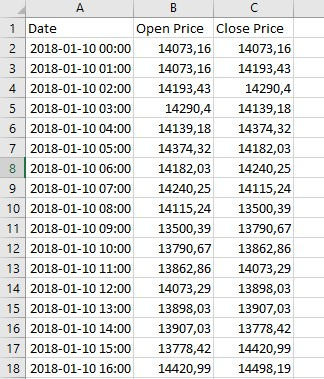
\includegraphics[width=.4\textwidth]{bitcoin}
	\caption{Bitcoin-Kursverlauf}
	\label{fig:bitcoin-course}
\end{figure}

Den Bitcoin--Kursen werden im Rahmen dieser Arbeit Tweets gegen\"ubergestellt. Ein Tweet hat maximal 280 Zeichen. In Abbildung \ref{fig:tweet} ist ein Beispiel für einen solchen Tweet zu sehen. 

\begin{figure}[htb]
	
\includegraphics[width=.5\textwidth]{tweet}
	\caption{Beispiel-Tweet}
	\label{fig:tweet}
\end{figure}

Um eine repr\"asentative Stichprobe zu haben, wurden knapp 120.000 englischsprachige Tweets untersucht. Neben dem Text eines Tweets, werden au{\ss}erdem Informationen \"uber denjenigen ausgelesen, der den Tweet verfasst hat, wann diese Kurznachricht verfasst wurde, eine eindeutige Identifikationsnummer, retweets und jede Menge andere Informationen. F\"ur diese Arbeit wurde jedoch nur das Erstellungsdatum und der Text eines Tweets gesammelt. Allgemein wurden nur Nachrichten aufgezeichnet, in denen die Zeichen: \textit{Bitcoin}, \textit{\#Bitcoin} und \textit{cryptocurrency} vorkommen.
Außerdem sind nur Tweets erfasst worden, die innerhalb der USA und einem Gro{\ss}teil von Kanada ver\"offentlicht wurden.
Da die Sentiment-Analyse am effizientesten funktioniert, wenn alle zu untersuchenden Texte in einer Sprache sind, wurde mit Hilfe der Bibliothek \enquote{TextBlob\footnote{Siehe http://textblob.readthedocs.io/en/dev/ .}} f\"ur jeden einzelnen Tweets die entsprechende Sprache ermittelt. Alle Nachrichten, die nicht in der Sprache Englisch waren, wurden daraufhin aus dem Datensatz entfernt.

\subsection{Methode}
Spark xyz ...

\subsection{Auswertung}
Die Meinung von Twitternutzern ist dem Bitcoin--Kurs in Abbildung \ref{fig:result} gegen\"ubergestellt. Die verschiedenen Tweets wurden mit Hilfe der Sentimentanalyse in negative, neutrale und positive Nachrichten unterteilt und in den S\"aulen farblich gekennzeichnet. Die H\"ohe der S\"aulen sentspricht der Anzahl an Nachrichten, die innerhalb eines Zeitintervalls von einer Stunde registriert wurden. Hohe S\"aulen weisen somit auf viele Nachrichten hin, während flache S\"aulen f\"ur wenig Twitter-Meldungen zum Thema Bitcoin stehen. 
Zus\"atzlich ist der Trend des Bitcoin-Kurses aufgetragen. Der jeweilige Wert wurde als Differenz aus Opening- und Closing-Betrag, wie in Abbildung \ref{fig:bitcoin-course} zu sehen, bestimmt. Ein positiver Wert entspricht somit einem steigenden Kursverlauf, ein negativer Wert entsprechend einem fallenden.

\begin{figure}[htb]
	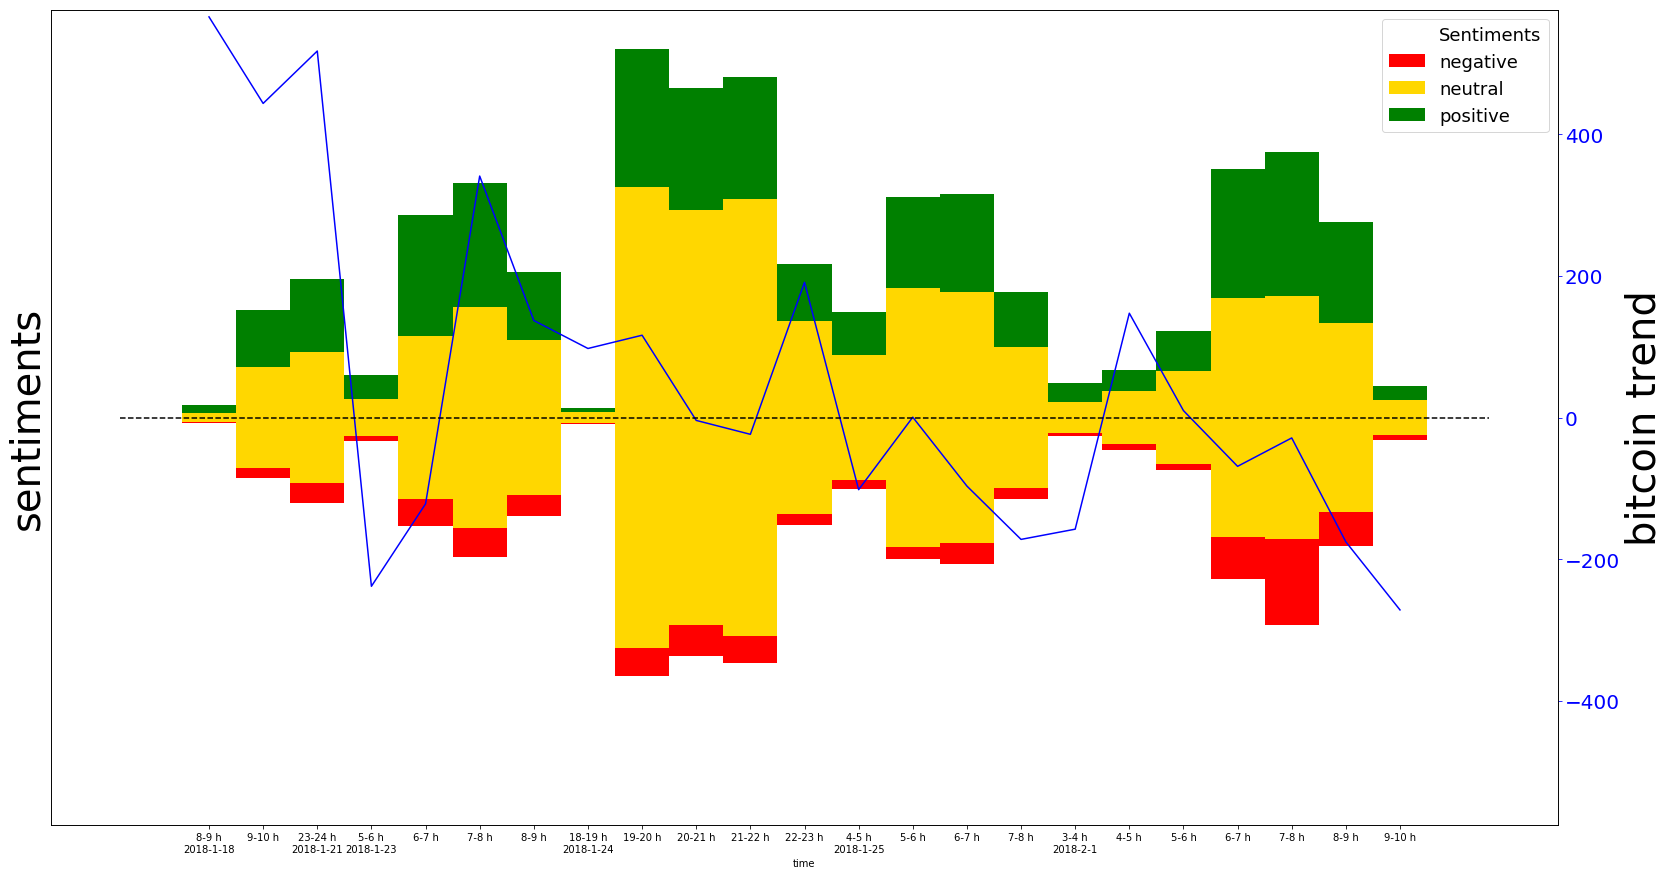
\includegraphics[width=\textwidth]{result}
	\caption{\"Ubersicht der Auswertungsergebnisse. Die blaue Kurve entspricht dem Bitcon-Trend. Die farblich unterteilten S\"aulen stellen die Anzahl an Meinungen dar, die den Clustern positiv (gr\"un), neutral (gelb) und negativ (rot) dar. Die S\"aulenh\"ohe steht f\"ur die Anzahl an Nachrichten pro Stunde.}
	\label{fig:result}
\end{figure}

Es ist zu beachten, dass die dargestellte Zeitachse nicht kontinuierlich verläuft. Viel mehr wurden pro Datum nur Nachrichten aus wenigen Stunden extrahiert. Dieses Verhalten ist auf die Bibliothek \enquote{tweepy\footnote{Siehe http://www.tweepy.org/ .}} zur\"uckzuf\"uhren, mit deren Hilfe die Tweets heruntergeladen wurde. Auf Grund der limitierten Downloadrate bei Twitter und den Einstellungen der Bibliothek wurden Anstelle des gew\"unschten Zeitraums vom 10.01.2018 -- 01.02.2018 lediglich Daten weniger, kurzer Zeitabschnitte heruntergeladen.\\
Aus den vorhandenen Daten lassen sich trotzdem einige Ergebnisse ableiten. 
\begin{itemize}
	\item Wie zu erwarten, ist die Anzahl der Meldungen in den fr\"uhen Morgenstunden geringer als am Abend.
	\item Der Anteil der neutralen Meldungen ist auffallend hoch. 
	\item Es gibt im Allgemeinen mehr positive Tweets zum Thema Bitcoin als negative.
	\item Der Bitcoin-Trend ist am 18.01. und am 21.01.2018 positiv. Zu den jeweiligen Zeitpunkten wurden jedoch nur verh\"altnism\"assig wenig Tweets registriert.
	\item Am 24.01.2018 ist das Interesse am Bitcoin deutlich gestiegen.
	\item Der negative Trend am 01.02.2018 wurde von mehr negativen Tweets begleitet, als zu allen anderen betrachteten Zeitpunkten. Jedoch ist auch die Anzahl der positiven Nachrichten gestiegen.
\end{itemize}

Insgesamt l\"asst sich kein Zusammenhang zwischen den Bitcoin-Trend und den Twitter-Nachrichten erkennen. Dies ist zum einen auf die geringe Stichprobe und die unregelm\"a{\ss}igen Zeitpunkte der Twitterdaten zur\"uckf\"uhren. Zum anderen deuten die vielen, als neutral eingestuften Meldungen darauf hin, dass der von \textit{TextBlob} verwendete Klassifikator nicht ausreichend gut auf die Problemstellung angepasst ist. 



%TODO:  Performance???

\textcolor{red}{Was ist mit Performance?}

\subsection{Ausblick}

andere Daten ...
konsistente Daten ...

\end{document}
